\chapter{Regularization}
% Authors: Liangzhi Li (editor), Lekha Iyengar, Subhadarshi Panda, 04/02/19.
\section{Problem}
We attempt to study the effect of L1 regularization,L2 regularization and Dropout in sentiment analysis of IMDB dataset. We split our data into training (17500 samples), valiation (7500 samples) and test set(2500 samples).

\section{Data processing}
We follow the following steps while processing the IMDB dataset
\begin{itemize}
    \item[1)] Tokenization: break sentence into individual words
    \begin{itemize}
        \item Before: "PyTorch seems really easy to use!"
        \item After: ["PyTorch", "seems", "really", "easy", "to", "use", "!"]
    \end{itemize}
    \item[2)] Building vocabulary: build an index of words associated with unique numbers
    \begin{itemize}
        \item Before: ["PyTorch", "seems", "really", "easy", "to", "use", "!"]
        \item After: {"Pytorch: 0, "seems": 1, "really": 2, ...}
    \end{itemize}
    We use a vocabulary of 1000 words in this example
    \item[3)] Convert to numerals: map words to unique numbers (indices)
    \begin{itemize}
        \item Before: {"Pytorch: 0, "seems": 1, "really": 2, ...}
        \item After: [0, 1, 2, ...]
    \end{itemize}
    \item[4)] Embedding look-up: map sentences (indices now) to fixed matrices 
    \begin{itemize}
        \item  [[0.1, 0.4, 0.3], [0.8, 0.1, 0.5], ...]
    \end{itemize}
\end{itemize}

\section{Architecture}
We use a Feed-forward neural network(FNN) for our task. (Not RNN/LSTM/GRU). FNN does not contain any cycles or loops in the network. There are no feedback connections in which outputs of the model are fed back. It cannot handle flexible sequence lengths so we have to fix the length of the input. We use a 3 layer FNN where the first layer is the embedding layer. This is followed by a hidden layer with RelU activation. We have a third output layer. We apply a sigmoid function to our output so that our loss doesn't have to go through sigmoid again.
There are two sentiments for a review - negative or positive. This is a binary classification problem so Binary Cross Entropy loss (BCE loss) is used.

\section{Experiments}
We experiment with the following regularizations in the classification problem:
\begin{itemize}
    \item No regularization
    \item Add L1 regularization
    \item Add L2 regularization
    \item Add Dropout
\end{itemize}
When no regularization is applied, the network overfits the training data and the validation loss is much larger than the training loss. When we apply L1, L2 or Dropout regularization, the validation loss is comparable to the training loss and the network does not overfit anymore.

\begin{figure}
    \centering
    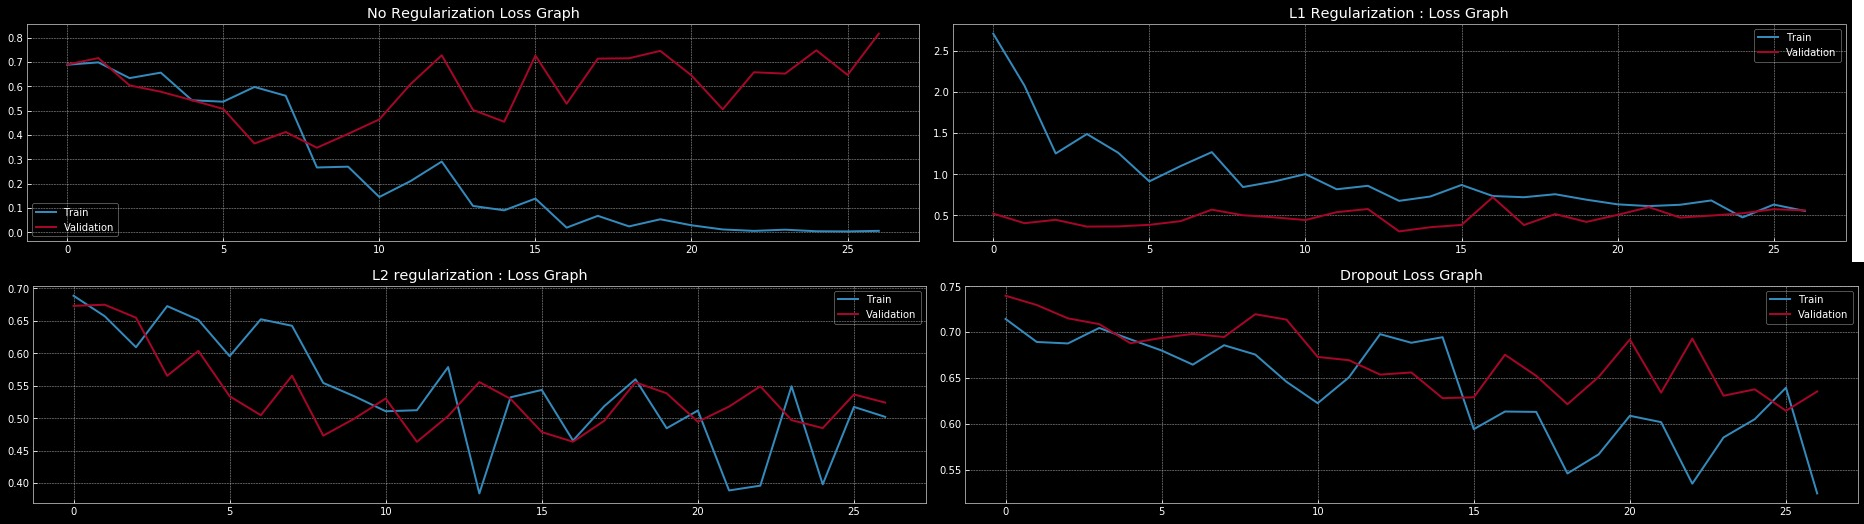
\includegraphics[scale=0.25]{labs/09/images/merged_loss_graph.png}
        \caption{Loss Graph}
        \label{fig:Loss Graph}
\end{figure}

\begin{figure}
    \centering
    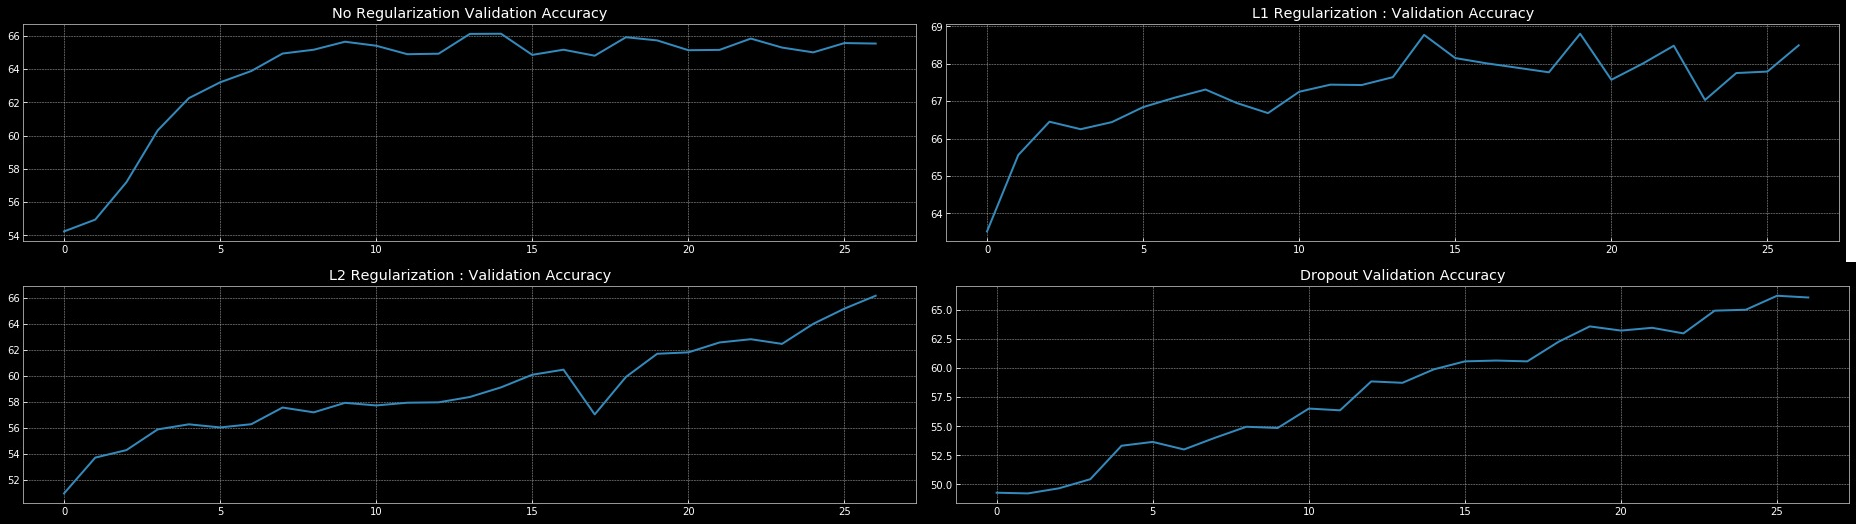
\includegraphics[scale=0.25]{labs/09/images/merged_acc.png}
        \caption{Validation accuracy}
        \label{fig:Validation accuracy}
\end{figure}

We see that when we apply dropout or no regularization to the network, the weights are more distributed. For L1 and L2 regularization though, most of the weights are close to 0. The L2 weights distribution is more spread out than L1 as it is like a Gaussian distribution, while L1 weights are like Laplacian distribution.

\begin{figure}
    \centering
    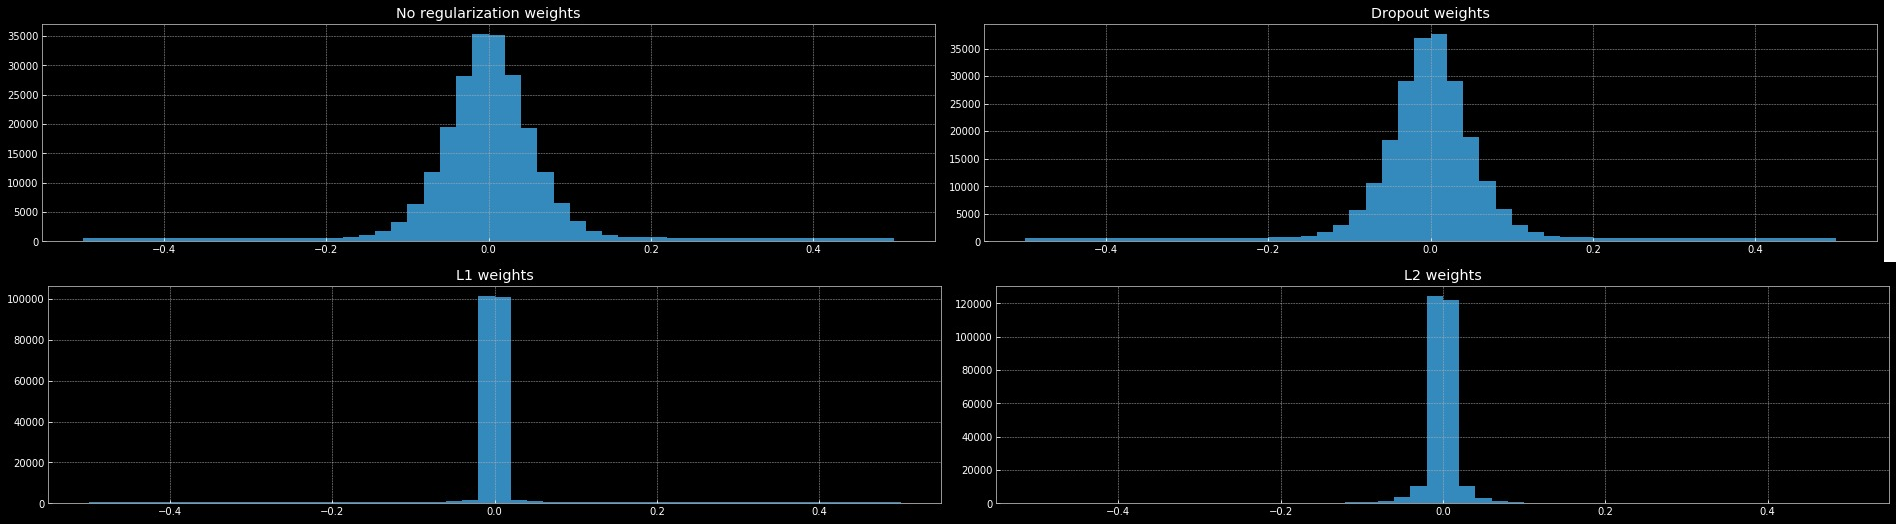
\includegraphics[scale=0.25]{labs/09/images/merged_weights_hist.png}
        \caption{Weights distribution for different regularizations }
        \label{fig:Weights distribution for different regularizations}
\end{figure}

\begin{figure}
    \centering
    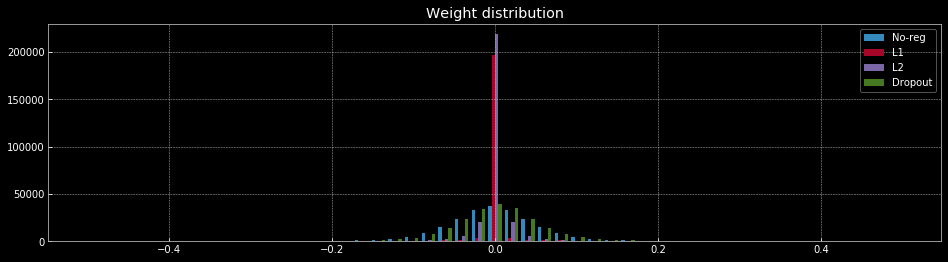
\includegraphics[scale=0.3]{labs/09/images/weights_dist.png}
        \caption{Weights distribution comparison}
        \label{fig:Weights distribution comparison}
\end{figure}